\documentclass[conference]{IEEEtran}
\IEEEoverridecommandlockouts

\usepackage{cite}
\usepackage{amsmath,amssymb,amsfonts}
\usepackage{algorithmic}
\usepackage{graphicx}
\usepackage{float}
\usepackage{textcomp}
\usepackage{xcolor}
\usepackage{makecell}
\usepackage{microtype}
\usepackage{multirow}
\def\BibTeX{{\rm B\kern-.05em{\sc i\kern-.025em b}\kern-.08em
    T\kern-.1667em\lower.7ex\hbox{E}\kern-.125emX}}

% FiLM conditioning paper citation + justification???
% rewrite discussion better
% conclusion
% hdf5 diagram

\begin{document}

\title{State of Health Estimation Using a Novel Dataset Under Extreme Temperature and Aging Conditions}

\author{\IEEEauthorblockN{1\textsuperscript{st} Sahar Qaadan}
	\IEEEauthorblockA{\textit{Department of Mechatronics Engineering} \\
		\textit{German Jordanian University}\\
		Madaba JO-11180, Jordan \\
		sahar.qadan@gju.edu.jo}
	\and
	\IEEEauthorblockN{2\textsuperscript{nd} Yousef Alfoqaha}
	\IEEEauthorblockA{\textit{Department of Computer Engineering} \\
		\textit{German Jordanian University}\\
		Madaba JO-11180, Jordan \\
		y.mustafa1@gju.edu.jo}
}

\maketitle

\begin{abstract}
	Accurate State of Health estimation in electric vehicle battery management systems is critical for operational safety. However, existing public benchmark datasets restrict model evaluation to narrow ambient temperatures and constant-current charging phases. To address this gap, we evaluate a baseline diagnostic estimator on a novel multi-protocol degradation dataset comprising eight Samsung INR21700-50E lithium-ion cells cycled across extreme temperatures ($-20^\circ\text{C}$ to $45^\circ\text{C}$) under realistic driving profiles, including WLTC, HPPC, pulse, and constant discharge segments. The proposed baseline framework combines 1D Convolutional Neural Networks for spatial feature extraction, Feature-wise Linear Modulation (FiLM) for ambient temperature conditioning, a Bidirectional Gated Recurrent Unit (BiGRU) for temporal modeling, and additive attention pooling. Evaluated on holdout cells across 14.2 million timesteps, the model achieves an overall SoH estimation error of $1.6\%$ ($\text{RMSE} = 0.016$, $R^2 = 0.96$). Furthermore, unfreezing the attention pooling head during fine-tuning on the Oxford Battery Degradation Dataset demonstrates cross-dataset transferability, reducing fine-tuned error to $0.8\%$ ($\text{RMSE} = 0.008$, $R^2 = 0.99$). Stratified Permutation Feature Importance confirms that current and voltage drive predictive performance, aligning with fundamental electro-chemical degradation mechanics.
\end{abstract}

\begin{IEEEkeywords}
	State of Health Estimation, Machine Learning, Lithium-Ion Batteries, Benchmark Dataset
\end{IEEEkeywords}

\section{Introduction}
With the electric vehicle (EV) market share surpassing 20\% of new global car sales \cite{iea_ev_outlook_2024}, battery management systems (BMS) in EVs rely on accurate state of health (SoH) estimations to ensure a margin of safety in maintaining critical vehicle components.
While SoH, in the capacity sense, is defined as $\mathrm{SOH}_C = C / C_{\mathrm{init}}$ \cite{birkl2017degradation}, microscopic manufacturing variations cause each lithium-ion battery (LiB) to follow a highly non-linear degradation trajectory; this makes tracking SoH a non-trivial task, especially in realistic driving scenarios.
Data-driven approaches typically employ diagnostic frameworks for real-time EV monitoring \cite{hu2020battery, lipu2023data}; by extracting instant features from available charge-discharge windows, they dynamically track sudden non-linear aging mechanisms like solid electrolyte interphase (SEI) layer growth and lithium plating as they occur \cite{okane2022degradation}.

Recent diagnostic models combine convolutional neural networks (CNN) for spatial feature extraction with recurrent neural networks (RNN), such as Long Short-Term Memory (LSTM) \cite{li2025anode, chen2023cnnlstm} or Gated Recurrent Units (GRU) \cite{xia2023bigru, chen2023skdan}, to model temporal dependencies common in LiB degradation.
These networks frequently integrate attention mechanisms to weight cycle data \cite{wei2023dualattn, chen2023skdan} and utilize support vector machines (SVM) or support vector regression (SVR) for final SoH regression \cite{zhang2025woavmd, li2025issasvr}.

Because generating battery degradation data is a laborious and time-consuming process, the vast majority of these models are trained and benchmarked on open-datasets such as NASA Ames \cite{saha2007battery}, Oxford \cite{birkl2017oxford}, CALCE \cite{pecht2011calce}, TJU \cite{wang2024tju}, and HUST \cite{li2021hust}.
While these datasets offer varied cell chemistries, they restrict model evaluation to constant-current (CC) charging phases and narrow ambient temperatures.
Thus, to complement existing benchmark datasets, a multi-protocol LiB degradation dataset was developed in collaboration with the University of Wuppertal \cite{uni_wuppertal_ees}.
This dataset comprises 8 Samsung INR21700-50E LiBs \cite{samsung_50e_spec}, which were cycled across a wide temperature spectrum (-20°C to 45°C) using a combination of realistic operational protocols, including the Worldwide Harmonised Light Vehicles Test Cycle (WLTC) \cite{wltc_unece}, Hybrid Pulse Power Characterization (HPPC) \cite{hppc_usabc}, pulse, and CC segments.

To establish a benchmark baseline, evaluation was performed on a diagnostic estimator combining CNN, BiGRU, and attention pooling layers.
We evaluate this baseline across the dataset's temperature bands and protocols, and verify its cross-dataset transferability by fine-tuning it on the Oxford Battery Degradation Dataset.
A comparative summary of public battery datasets and estimation frameworks is provided in Table \ref{tab:related_works}.

\begin{table*}[htbp]
	\caption{Comparison of Benchmark Battery Degradation Datasets and Diagnostic Estimation Frameworks}
	\label{tab:related_works}
	\centering
	\small
	\begin{tabular}{l l c c l}
		\hline
		\textbf{Dataset / Study} & \textbf{Cell Form / Chemistry}          & \textbf{Temperature Range} & \textbf{Discharge Protocols} & \textbf{Baseline Evaluated} \\
		\hline
		NASA Ames                & \makecell[l]{18650 Cylindrical                                                                                                    \\ LCO-NCA} & $20^\circ\mathrm{C}$ to $30^\circ\mathrm{C}$ & CC & SVR, LSTM, ANODE \\
		\hline
		Oxford Dataset 1         & \makecell[l]{Pouch / LCO                                                                                                          \\ ($740\,\mathrm{mAh}$)} & $40^\circ\mathrm{C}$ (Static) & CC & Dual-Attn Graph CNN \\
		\hline
		HUST Dataset             & \makecell[l]{18650 Cylindrical                                                                                                    \\ LFP} & Uncontrolled Ambient & Multi-step CC & Deep Transfer Learning \\
		\hline
		\textbf{This Work}       & \makecell[l]{\textbf{21700 Cylindrical}                                                                                           \\ \textbf{NMC ($5.0\,\mathrm{Ah}$)}} & \textbf{$-20^\circ\mathrm{C}$ to $45^\circ\mathrm{C}$} & \textbf{WLTC, HPPC, Pulse, CC} & \textbf{CNN+BiGRU+Attn} \\
		\hline
	\end{tabular}
\end{table*}

\section{Data Processing}

\subsection{Dataset}
The dataset was obtained from the Scienlab SL1007A charge--discharge testing platform, where eight Samsung INR21700-50E lithium-ion cells (NMC chemistry, rated capacity $C_{\mathrm{init}} = 5.0\,\text{Ah}$, voltage range $2.5$--$4.2\,\text{V}$, maximum rated C-rates of 2C charge / 4C discharge) were cycled from fresh SoH levels to beyond end-of-life \cite{scienlab_sl1007a}.
Telemetry of each cell was recorded using Measurement and Control Units (MCU) and exported as ASAM Measurement Data Format (MF4) files \cite{asam_mdf4}.

Initial measurements were taken across CC, pulse, HPPC, and WLTC protocols (Fig. \ref{fig:protocols}), with ambient temperatures at $-20$, $-10$, $-5$, $0$, $10$, $25$, and $40^{\circ}\text{C}$. CC and pulse protocols were tested at $0.1$, $0.5$, $1.0$, and $2.0$C. Cyclic aging was then performed using CC discharge at $1.0$C and $25^{\circ}\text{C}$. Post aging measurements were taken using the same procedure as the initial phase (excluding WLTC). The distribution of cycles across temperature bands and discharge protocols is shown in Table \ref{tab:temp_protocol_matrix}.

\begin{figure}
	\centerline{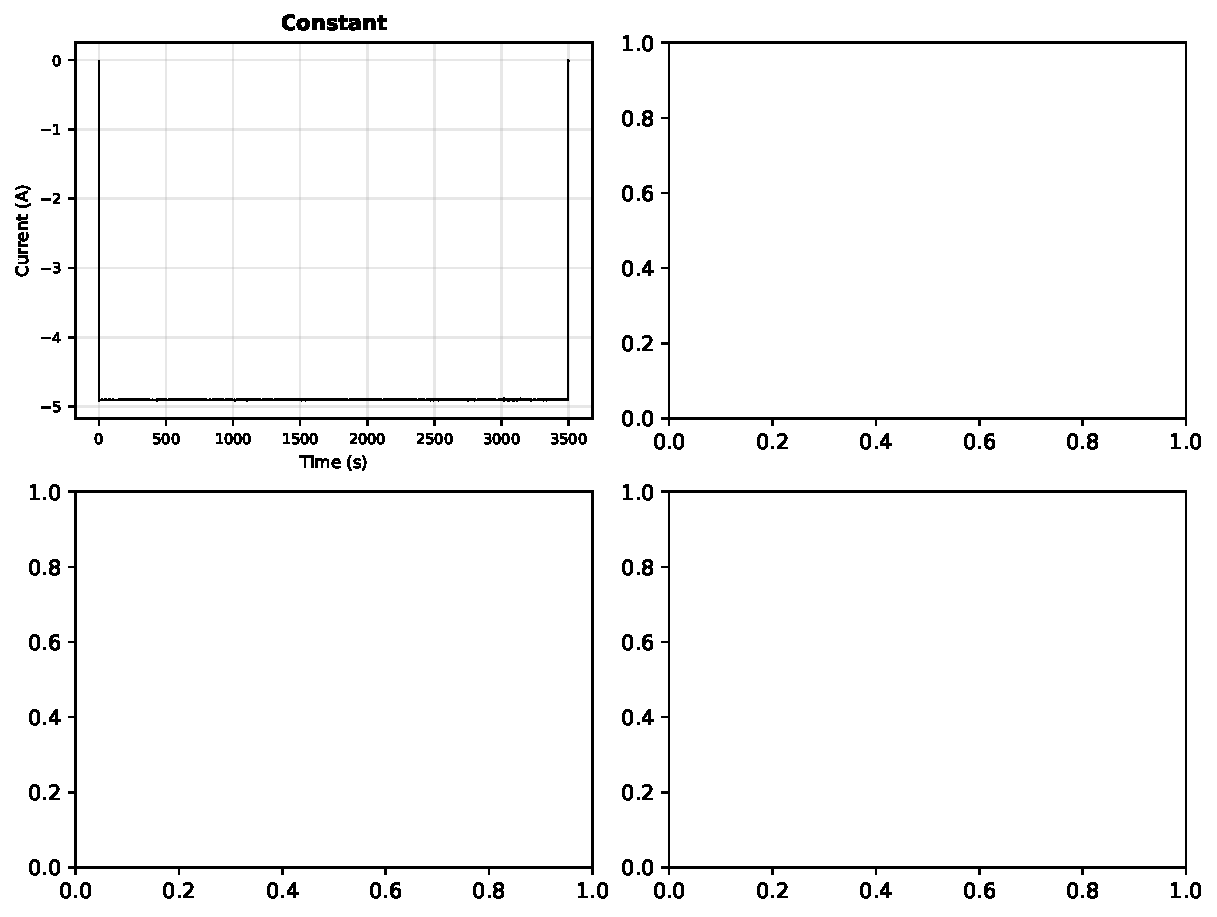
\includegraphics[width=\columnwidth]{discharge_protocols.pdf}}
	\caption{Discharge profiles for the four test protocols: CC, Pulse, HPPC, and WLTC.}
	\label{fig:protocols}
\end{figure}

\begin{table}[H]
	\caption{TEMPERATURE BAND DISTRIBUTION}
	\label{tab:temp_phase_matrix}
	\begin{center}
		\footnotesize
		\begin{tabular}{lccccccc}
			\hline
			\textbf{Phase} & $\mathbf{-20}$ & $\mathbf{-10}$ & $\mathbf{-5}$ & $\mathbf{0}$ & $\mathbf{10}$ & $\mathbf{25}$ & $\mathbf{40}$ \\
			\hline
			Initial        & 38             & 30             & 6             & 74           & 14            & 127           & 59            \\
			Aging          & 0              & 0              & 0             & 0            & 0             & 792           & 0             \\
			Post-Aging     & 39             & 50             & 0             & 54           & 8             & 95            & 56            \\
			\hline
			\textbf{Total} & \textbf{77}    & \textbf{80}    & \textbf{6}    & \textbf{128} & \textbf{22}   & \textbf{1014} & \textbf{115}  \\
			\hline
		\end{tabular}
	\end{center}
\end{table}


\subsection{Pre-processing Pipeline}
As per the dataset engineer's advice, voltage ($V$), current ($I$), temperature ($T$), and ambient temperature ($T_{amb}$) are primary channels recorded from the test platform's sensors.
A script was used to filter discharge periods using start/end signals provided by the testing platform. Raw cycles recorded at up to $1\text{~kHz}$ ($1\text{~ms}$) were downsampled to $1\text{~Hz}$ ($1\text{~s}$).
For each cycle, the mean value of $T_{amb}$ was taken since it is a fixed condition set by the test platform.

The MF4 cycles were then consolidated into a single Hierarchical Data Format (HDF5) \cite{hdf5} file using \texttt{h5py} \cite{h5py}. This structure allows $V$, $I$, and $T$ matrices to be stored as $N$-dimensional arrays. Furthermore, metadata including the discharge protocol, testing phase, ambient temperature, discharge rate, date-time, cycle index, and target SoH are embedded directly into each cycle as scalar attributes. Consolidating the raw files into a single HDF5 container eliminates MF4 file-handling overhead, provides $O(1)$ random-access indexing for data loading, and presents a uniform interface for model training.


\begin{figure}[H]
	\centerline{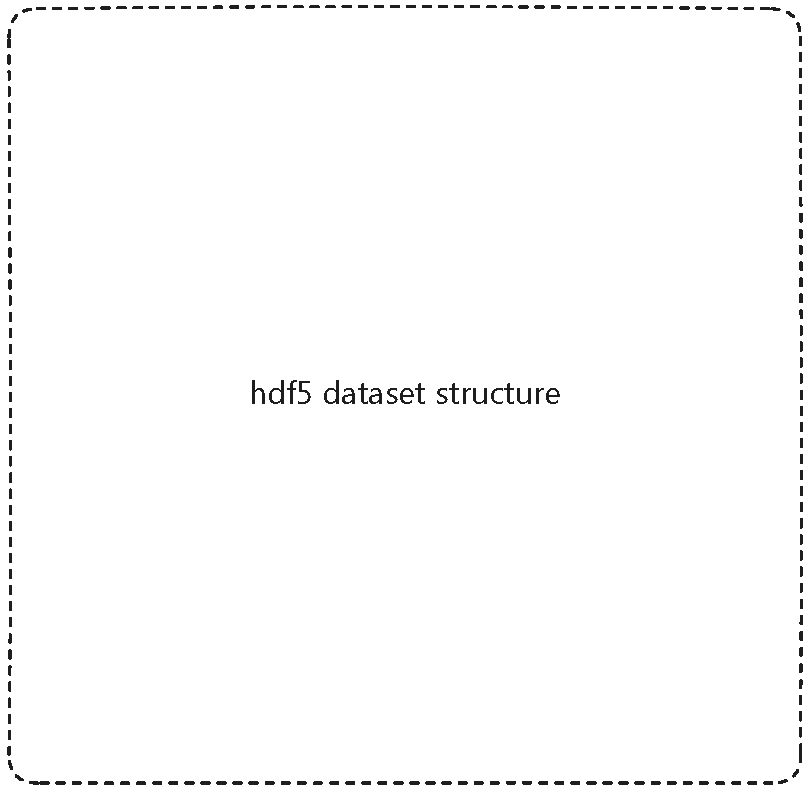
\includegraphics[width=\columnwidth]{dataset_structure.pdf}}
	\caption{HDF5 dataset structure of MCUs, cycles, and attributes.}
	\label{fig:dataset_structure}
\end{figure}

\subsection{SoH Labeling}
Raw SoH for each discharge cycle was computed via Coulomb counting:

\begin{equation}
	\text{SoH}_{\text{raw}} = \frac{\int_{t_{\text{start}}}^{t_{\text{end}}} |I(t)| \, dt}{C_{\text{nom}}}
\end{equation}

Measured capacity depends on discharge rate and $T_{\text{amb}}$, so raw SoH is not directly comparable across cycles. Discharge cycles at $1\text{C}$ and $25^\circ\text{C}$, the only condition common to all phases, are used as reference points. A 4th degree polynomial is fit over cycle index to these reference points, giving a per-MCU SoH trajectory (Fig. \ref{fig:soh_trajectories}). Reference-point SoH ranges and cycle counts are given in Table \ref{tab:mcu_soh_summary}.


\begin{figure}
	\centerline{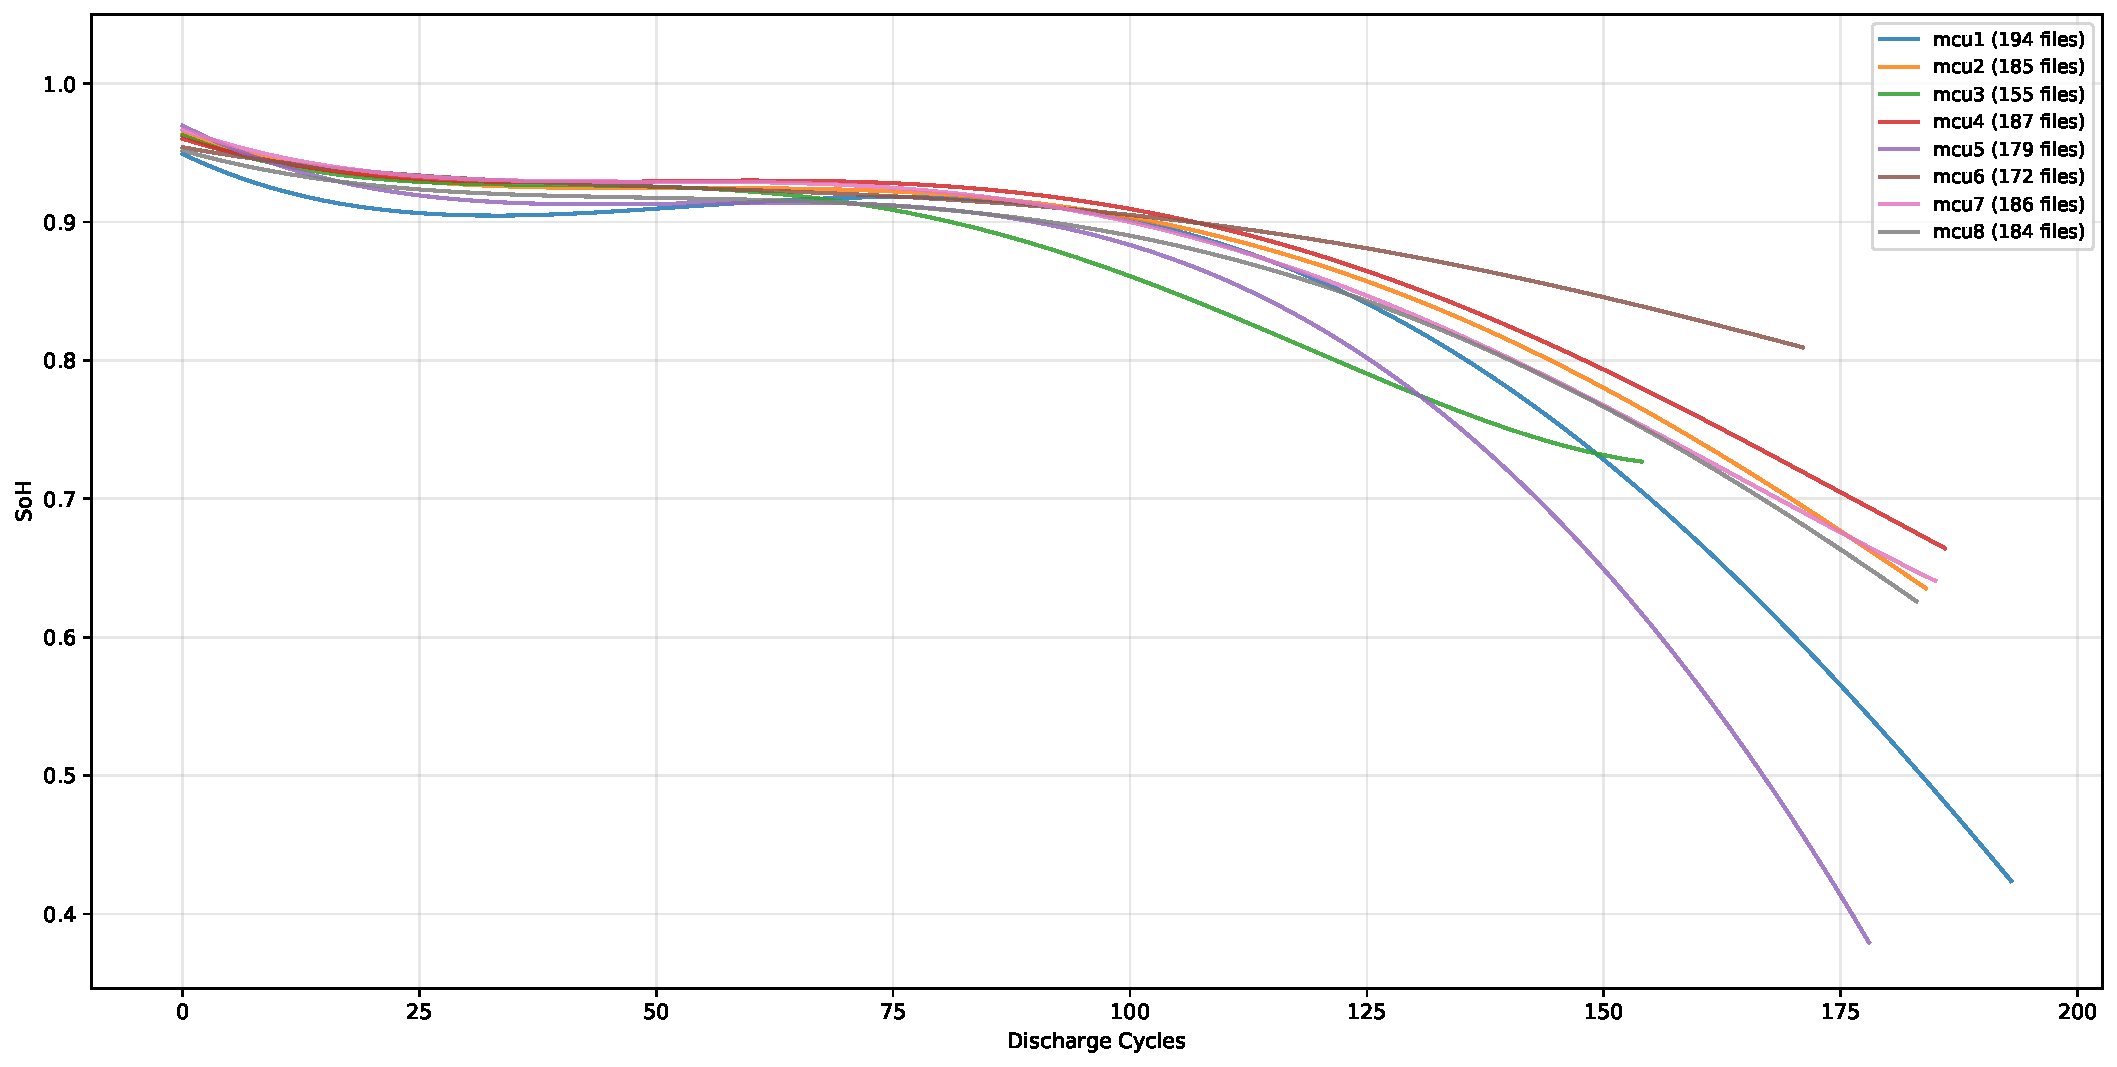
\includegraphics[width=\columnwidth]{soh_trajectories.pdf}}
	\caption{Fitted SoH trajectories for all eight MCUs across their full discharge cycle histories.}
	\label{fig:soh_trajectories}
\end{figure}

\begin{table}[H]
    \caption{MCU SOH RANGE AND CYCLE COUNT}
    \label{tab:mcu_soh_summary}
    \begin{center}
        \footnotesize
        \begin{tabular}{lcc}
            \hline
            \textbf{MCU} & \textbf{SoH Range (\%)} & \textbf{Cycles} \\
            \hline
            1 & $94.9$--$46.5$ & 194 \\
            2 & $96.4$--$66.8$ & 185 \\
            3 & $96.2$--$74.0$ & 155 \\
            4 & $96.0$--$69.7$ & 187 \\
            5 & $97.0$--$40.2$ & 179 \\
            6 & $95.4$--$82.6$ & 172 \\
            7 & $96.7$--$66.5$ & 186 \\
            8 & $95.2$--$65.5$ & 184 \\
            \hline
        \end{tabular}
    \end{center}
\end{table}


\subsection{Feature Scaling}

Z-score standardization is sensitive to extreme temperature and aging conditions, where wide swings are valid.
Instead, an unclipped robust scaling approach \cite{han2011data} maps the $1^{\text{st}}$ and $99^{\text{th}}$ percentiles ($p_{01}$, $p_{99}$) to $[-1, 1]$, normalizing the 14,262,367 time steps for training stability.
Mean and standard deviation per feature are given in Table \ref{tab:feature_stats}.

\begin{equation}
	x_{\text{norm}} = \frac{x - p_{01}}{p_{99} - p_{01}}
\end{equation}

\begin{table}[H]
    \caption{FEATURE STATISTICS}
    \label{tab:feature_stats}
    \begin{center}
        \begin{tabular}{lcc}
            \hline
            \textbf{Feature}                         & \textbf{Mean ($\mu$)} & \textbf{Std. Dev. ($\sigma$)} \\
            \hline
            Voltage ($V$)                            & 3.6001                & 0.3250                        \\
            Current ($I$)                            & -1.5609                & 2.1850                        \\
            Cell Temperature ($T$)                   & 16.9842                & 18.0212                        \\
            Ambient Temperature ($T_{\text{amb}}$)   & 15.5569                & 18.0118                        \\
            Thermal Delta ($\Delta T_{\text{cell}}$) & 4.9908                & 3.3976                        \\
            State of Health ($\text{SoH}$)           & 0.8614                & 0.1089                        \\
            \hline
        \end{tabular}
    \end{center}
\end{table}


\section{Methodology}

\subsection{Problem Formulation}
Given a sequence of $V$, $I$, and $T$ over a discharge cycle, conditioned on $T_{\text{amb}}$, an estimator function $f(\cdot)$ predicts the cell's $\text{SoH}$:

\begin{equation}
	\widehat{\text{SoH}} = f(V, I, T \mid T_{\text{amb}})
\end{equation}

\subsection{Estimator Architecture}

As illustrated in Fig. \ref{fig:architecture}, A window of sequences $V$, $I$, and $T$ of length $N$ pass through a stem 1D Convolutional Neural Network (1D-CNN) layer followed by two strided 1D-CNN blocks ($4\times$ base channels; GroupNorm, LeakyReLU, dropout), followed by Feature-wise Linear Modulation (FiLM) conditioning on $T_{\text{amb}}$:

\begin{equation}
	\text{FiLM}(h) = (1 + \gamma(T_{\text{amb}})) \odot h + \beta(T_{\text{amb}})
\end{equation}

where $\gamma$ and $\beta$ are learned affine parameters. The modulated features pass through a 2-layer bidirectional Gated Recurrent Unit (BiGRU). An additive attention mechanism then pools over the GRU output timesteps:

\begin{equation}
	\alpha_t = \frac{\exp(w^\top \tanh(W h_t))}{\sum_{\tau} \exp(w^\top \tanh(W h_\tau))}, \quad z = \sum_t \alpha_t h_t
\end{equation}

where $h_t$ is the BiGRU output at timestep $t$. The pooled representation $z$ is projected to a scalar SoH estimate.

\begin{figure*}
	\centering
	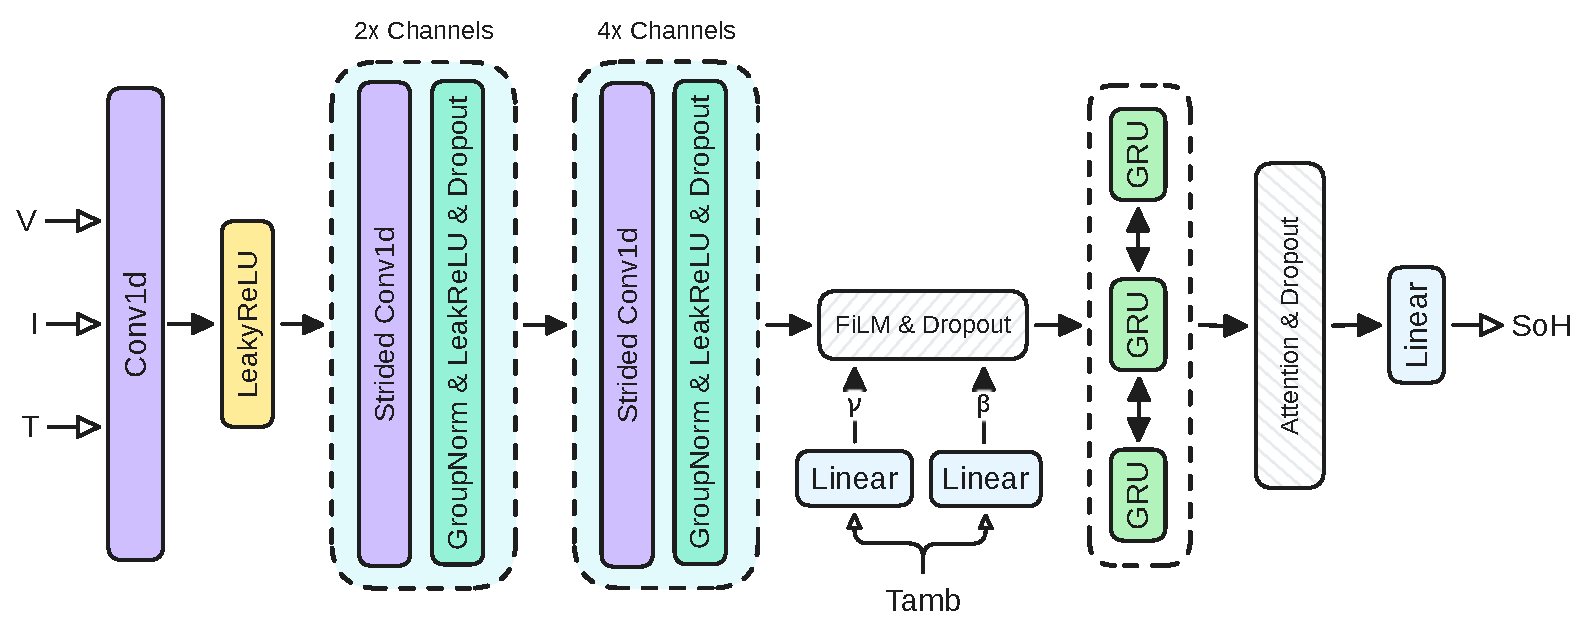
\includegraphics[width=\textwidth]{architecture.pdf}
	\caption{Model architecture: 1D-CNN blocks, BiGRU, and FiLM conditioning on $T_{\text{amb}}$.}
	\label{fig:architecture}
\end{figure*}


\subsection{Training Setup}

Raw input sequences (1,500 to 30,000 timesteps per cycle) were sliced into 1,500-timestep windows (15 minutes) with a 1,000-timestep stride. The model predicted the SoH for each window, and these predictions were averaged to produce a single SoH value per cycle.
The eight MCUs were split 6/1/1 into training, validation, and test sets.
MCUs 2 and 7 were held out for validation and testing, respectively, as their SoH range ($95.6$--$67.5\%$) falls within the training range ($97.4$--$42.3\%$). The validation set was shuffled once to break temporal symmetry between the initial, aging, and post-aging phases. The training set was shuffled every epoch.

In total, the training set comprised 1,071 cycles (7,227 windows), while the validation set contained 185 cycles (1,341 windows). All input sequences and conditions were normalized using robust min-max scaling. The Estimator's hyperparameters are given in Table \ref{tab:estimator_hparams}.

\begin{table}[H]
	\caption{ESTIMATOR HYPERPARAMETERS}
	\label{tab:estimator_hparams}
	\begin{center}
		\footnotesize
		\begin{tabular}{lc}
			\hline
			\textbf{Hyperparameter} & \textbf{Value} \\
			\hline
			Conv. base channels     & 64             \\
			Conv. kernel size       & 7              \\
			Conv. stride            & 2              \\
			GRU hidden size         & 128            \\
			GRU layers              & 2              \\
			Dropout                 & 0.2            \\
			LeakyReLU slope         & 0.2            \\
			\hline
		\end{tabular}
	\end{center}
\end{table}


The framework was implemented in PyTorch and accelerated on an NVIDIA RTX 5060ti 16Gb GPU. The model was trained using the AdamW optimizer (weight decay of $10^{-2}$) and a batch size of 128 windows to minimize the mean squared error (MSE) loss. The \texttt{ReduceLROnPlateau} scheduler was used on an initial learning rate of $2 \times 10^{-2}$, which decayed by a factor of $0.5$ (minimum $10^{-5}$) upon encountering a 15-epoch plateau in validation loss. Early stopping was used to halt training after 50 epochs without improvement, restoring the model weights that achieved the lowest validation loss.

\subsection{Results}

Evaluation was performed on the testing MCU across testing phases, temperature bands and discharge protocols (Table \ref{tab:temp_protocol_results}).
Most overall metrics derive from the aging phase, which achieves low error.
The initial phase reaches $1.3\%$ error (RMSE $0.015$).
Aging is the strongest phase ($R^2 = 0.94$, $1.1\%$ error, RMSE $0.011$).
Notably, Initial and Aging achieve similar metrics despite the former having far fewer cycles and greater protocol/temperature variance.
Post-Aging error rises to $3.0\%$ (RMSE $0.031$). Overall, $R^2 = 0.96$ and $1.6\%$ error across $62.8$--$96.2\%$ SoH.
The $40^{\circ}\text{C}$ band achieves a high fit among temperature slices ($R^2 = 0.98$, $1.5\%$ error), while $-20^{\circ}\text{C}$ trails behind with the lowest fit ($R^2 = 0.83$, $4.0\%$ error) and $-10^{\circ}\text{C}$ shows a strong fit among the higher-cycle bands ($R^2 = 0.98$, $2.4\%$ error).
$-20^{\circ}\text{C}$ spans $68.1$--$93.7\%$ at $R^2 = 0.83$ and $40^{\circ}\text{C}$ spans $66.8$--$95.1\%$ at $R^2 = 0.98$.
Across discharge protocols, (performance metrics) with each protocol spanning multiple temperature bands (Table~\ref{tab:temp_protocol_matrix}). Constant and HPPC achieve the highest fits ($R^2 = 0.97$ and $0.99$), and Pulse follows ($R^2 = 0.93$). WLTC has an $R^2$ of $0.10$, but this reflects $2$ cycles restricted to the Initial phase, giving a narrow SoH band ($92.1$--$95.3\%$) (Table~\ref{tab:mcu_soh_summary}).
The testing MCU's SoH trajectory with predicted points is shown in Fig.~\ref{fig:test_trajectory}.

\begin{table}[H]
    \caption{ESTIMATOR PERFORMANCE BY TEMPERATURE AND PROTOCOL}
    \label{tab:temp_protocol_results}
    \begin{center}
        \footnotesize
        \begin{tabular}{lcccccc}
            \hline
            \textbf{Slice} & \textbf{SoH (\%)} & \textbf{RMSE} & \textbf{MAE} & \textbf{R\textsuperscript{2}} & \textbf{\%Err} & \textbf{Cycles} \\
            \hline
            \multicolumn{7}{c}{\textbf{Temperature Bands}} \\
            $-20^{\circ}\text{C}$ & $68.5$--$93.7$ & 0.043 & 0.029 & $0.81$ & 3.9\% & 16 \\
            $-10^{\circ}\text{C}$ & $62.9$--$93.3$ & 0.037 & 0.031 & $0.86$ & 4.3\% & 18 \\
            $-5^{\circ}\text{C}$ & $92.6$--$92.6$ & 0.043 & 0.043 & -- & 4.7\% & 1 \\
            $0^{\circ}\text{C}$ & $64.3$--$94.0$ & 0.024 & 0.019 & $0.95$ & 2.4\% & 28 \\
            $10^{\circ}\text{C}$ & $69.8$--$92.8$ & 0.035 & 0.032 & $0.88$ & 4.1\% & 4 \\
            $25^{\circ}\text{C}$ & $65.7$--$96.1$ & 0.024 & 0.014 & $0.82$ & 1.6\% & 247 \\
            $40^{\circ}\text{C}$ & $67.1$--$95.0$ & 0.019 & 0.014 & $0.96$ & 1.7\% & 25 \\
            \hline
            \multicolumn{7}{c}{\textbf{Discharge Protocols}} \\
            Constant & $62.9$--$96.1$ & 0.027 & 0.016 & $0.86$ & 1.9\% & 246 \\
            HPPC & $68.5$--$92.9$ & 0.036 & 0.034 & $0.87$ & 4.2\% & 23 \\
            Pulse & $71.1$--$95.0$ & 0.016 & 0.013 & $0.97$ & 1.6\% & 67 \\
            WLTC & $92.4$--$95.2$ & 0.013 & 0.010 & $-0.17$ & 1.1\% & 3 \\
            \hline
            \textbf{Overall} & $\mathbf{62.9$--$96.1}$ & \textbf{0.026} & \textbf{0.016} & $\mathbf{0.89}$ & \textbf{2.0\%} & \textbf{339} \\
            \hline
        \end{tabular}
    \end{center}
\end{table}


\begin{figure}[H]
	\centerline{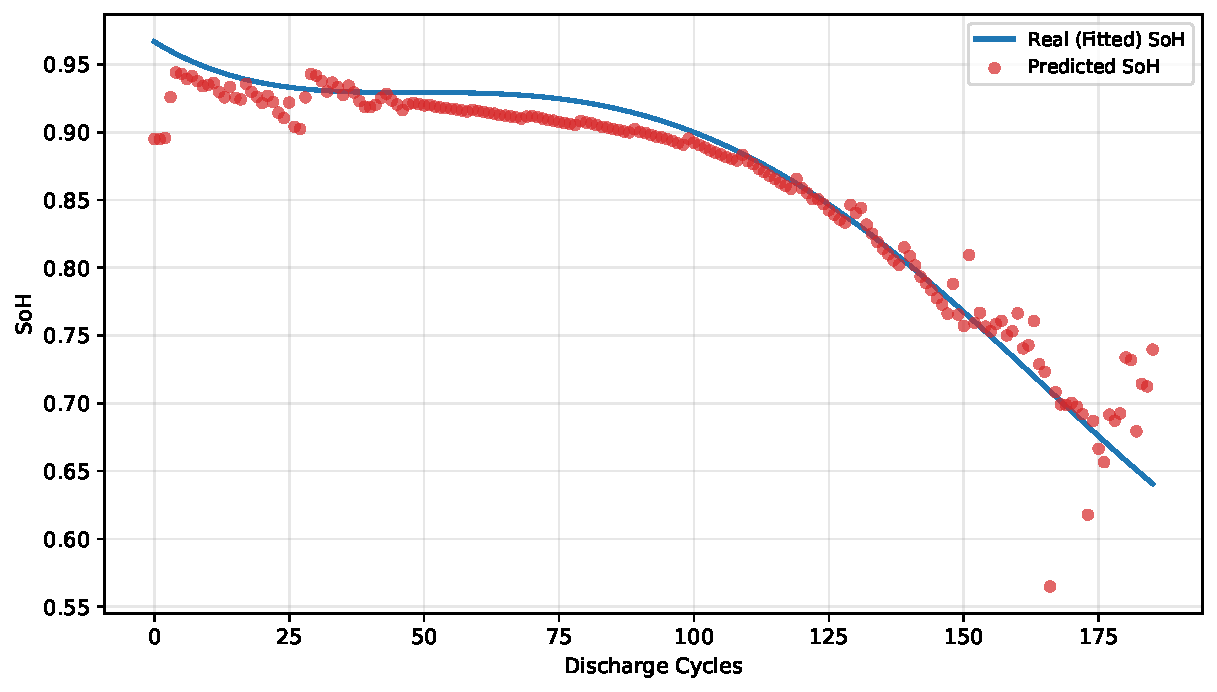
\includegraphics[width=\columnwidth]{test_trajectory.pdf}}
	\caption{Testing MCU SoH trajectory with predicted SoH points.}
	\label{fig:test_trajectory}
\end{figure}

\section{Cross-Dataset Validation}

\subsection{Oxford Battery Degredation Dataset 1}

The model was fine-tuned on the Oxford Battery Degradation Dataset 1 to evaluate cross-dataset transferability. The dataset comprises eight Kokam $740\,\text{mAh}$ LCO pouch cells (SLPB526495) aged under constant 1C discharge at $40^\circ\mathrm{C}$. This presents a severe domain shift in cell architecture, chemistry, and capacity relative to the Samsung INR21700-50E cylindrical cells ($5.0\,\text{Ah}$) used for primary training.
SoH labels were computed via Coulomb counting (1). SoH ranges for each cell are given in Table \ref{tab:oxford_soh_summary}.

\begin{table}[H]
	\caption{Oxford Cell SoH Range and Cycle Count}
	\label{tab:oxford_soh_summary}
	\centering
	\footnotesize
	\begin{tabular}{lcc}
		\hline
		\textbf{Cell} & \textbf{SoH Range (\%)} & \textbf{Cycles} \\
		\hline
		1             & $100.0$--$82.1$         & 115             \\
		2             & $100.0$--$81.4$         & 160             \\
		3             & $100.0$--$83.5$         & 124             \\
		4             & $100.0$--$82.9$         & 102             \\
		5             & $100.0$--$84.1$         & 143             \\
		6             & $100.0$--$83.0$         & 107             \\
		7             & $100.0$--$82.5$         & 171             \\
		8             & $100.0$--$81.9$         & 141             \\
		\hline
	\end{tabular}
\end{table}

\subsection{Fine-Tuning Setup}

The 1D-CNN, FiLM, and BiGRU layers were frozen, leaving only the attention pooling mechanism and output regression head open for fine-tuning. The eight cells were partitioned into a 6/1/1 split, allocating Cells 1--6 for fine-tuning, Cell 7 for validation, and Cell 8 for testing (Table~\ref{tab:oxford_soh_summary}). Feature scaling bounds, hyperparameter settings and shuffling strategy were kept identical to the primary training setup.

\subsection{Results}

Evaluating the model in a zero-shot setting yields severe performance degradation, resulting in an RMSE of $0.406$ ($46.8\%$ error) and an $R^2$ of $-36.66$ (Table~\ref{tab:oxford_results}).
However, unfreezing only the attention pooling mechanism and output regression head resolves this domain discrepancy. Upon fine-tuning, performance improves dramatically, achieving an RMSE of $0.008$, an MAE of $0.006$, an $R^2$ of $0.99$, and reducing the mean percentage error to $0.8\%$ across all 76 evaluation cycles.
As shown in Fig.~\ref{fig:oxford_trajectory}, in contrast to the zero-shot predictions, the fine-tuned predictions closely track ground-truth capacity fade.

\begin{table}[H]
    \caption{OXFORD DATASET PERFORMANCE: ZERO-SHOT VS. FINE-TUNED (EVALUATED ON HELD-OUT TEST CELLS)}
    \label{tab:oxford_results}
    \begin{center}
        \footnotesize
        \begin{tabular}{lcccccc}
            \hline
            \textbf{Model} & \textbf{SoH (\%)} & \textbf{RMSE} & \textbf{MAE} & \textbf{R\textsuperscript{2}} & \textbf{\%Err} & \textbf{Cycles} \\
            \hline
            Zero-Shot & $75.4$--$98.3$ & 0.376 & 0.371 & $-31.39$ & 43.2\% & 76 \\
            \textbf{Fine-Tuned} & $\mathbf{75.4$--$98.3}$ & \textbf{0.012} & \textbf{0.010} & $\mathbf{0.97}$ & \textbf{1.1\%} & \textbf{76} \\
            \hline
        \end{tabular}
    \end{center}
\end{table}


\begin{figure}[H]
	\centerline{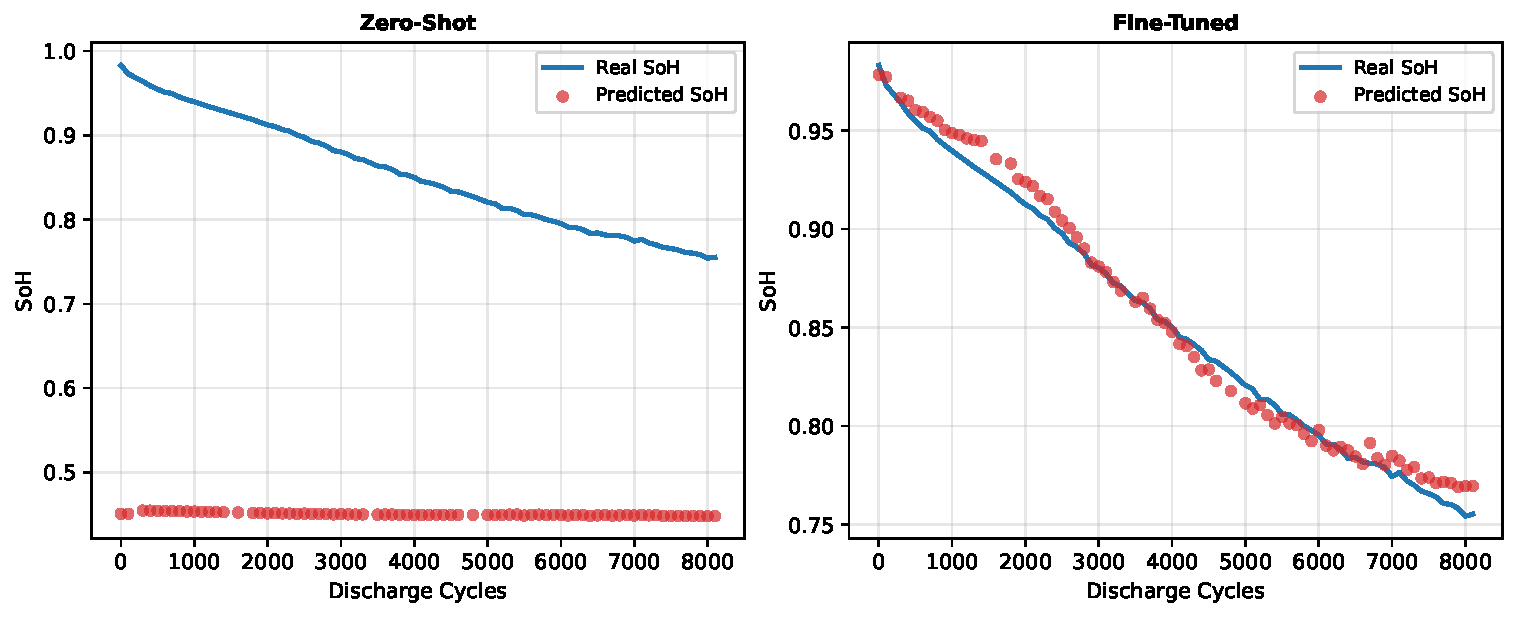
\includegraphics[width=\columnwidth]{oxford_trajectory.pdf}}
	\caption{Estimated versus ground-truth SoH trajectory on the testing cell for both zero-shot and fine-tuned scenarios.}
	\label{fig:oxford_trajectory}
\end{figure}


\section{Feature Interpretability}

\subsection{Permutation Feature Importance (PFI)}
PFI was used to measure which inputs the model relies on for its predictions. PFI shuffles one feature at a time across discharge cycles and measures the resulting drop in performance:
\begin{equation}
	\Delta \text{RMSE}_{j} = \text{RMSE}_{\text{perm}(j)} - \text{RMSE}_{\text{base}}, \quad j \in \{I, V, T, T_{amb}\}
\end{equation}

Shuffling was only done within the following controlled testing conditions: discharge protocol, ambient temperature, and discharge rate. This isolates the true importance of each feature from differences caused by the test setup itself.

\subsection{Results}
The stratified PFI results (Table~\ref{tab:pfi_results} and Fig.~\ref{fig:pfi_importance}) demonstrate that current ($I$) and voltage ($V$) are the primary drivers of model predictions across all protocols.

\begin{table}[H]
	\caption{Stratified PFI Results}
	\label{tab:pfi_results}
	\begin{center}
		\footnotesize
		\begin{tabular}{lrrrr}
			\hline
			\textbf{Feature} & \textbf{Constant} & \textbf{HPPC}    & \textbf{Pulse}   & \textbf{WLTC} \\
			\hline
			$I$              & +0.1037           & +0.1838          & \textbf{+0.1906} & +0.0194       \\
			$V$              & +0.0603           & \textbf{+0.1747} & +0.1268          & +0.0138       \\
			$T_{amb}$        & +0.0045           & +0.1383          & \textbf{+0.1563} & +0.0000       \\
			$T$              & \textbf{+0.0084}  & +0.0004          & -0.0029          & -0.0001       \\
			\hline
		\end{tabular}
	\end{center}
\end{table}


\begin{figure}[H]
	\centerline{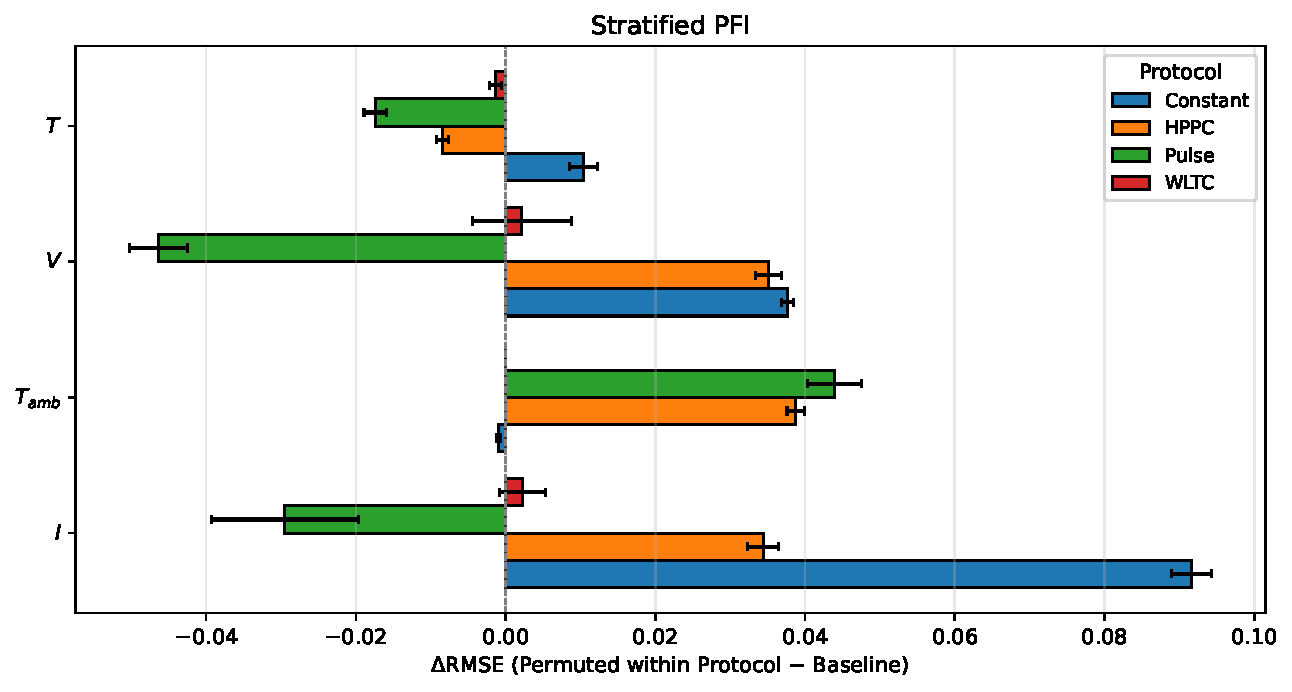
\includegraphics[width=\columnwidth]{pfi_importance.pdf}}
	\caption{Protocol-stratified Permutation Feature Importance ($\Delta\text{RMSE}$) across input channels ($I, V, T, T_{\text{amb}}$).}
	\label{fig:pfi_importance}
\end{figure}

\section{Discussion}
The Aging phase achieves the lowest error ($1.1\%$, $R^2 = 0.94$), likely
because its narrow test conditions, constant $1\text{C}$ discharge at
$25^\circ\text{C}$, produce a consistent waveform the CNN--BiGRU exploits
while still tracking the underlying SoH decline. The Initial phase shows a
negative $R^2$ ($-0.81$) despite a comparable RMSE ($0.015$); this is a
mathematical artifact of its narrow SoH range ($91.8$--$96.2\%$), where
limited target variance amplifies residual error rather than reflecting
poor fit, making RMSE and \%Err the more meaningful metrics here. The same
logic extends to temperature: $-20^\circ\text{C}$ trails all bands
($R^2 = 0.83$, $4.0\%$ error), but this reflects a $45^\circ\text{C}$ shift
from the $25^\circ\text{C}$ baseline, versus only $15^\circ\text{C}$ for the
$40^\circ\text{C}$ band ($R^2 = 0.98$), so the model is generalizing across
a substantially larger thermal gap than the headline numbers suggest.

The Oxford fine-tuning result supports this generalization at the
representation level. Zero-shot transfer fails outright (RMSE $= 0.406$,
$46.8\%$ error), consistent with the scale mismatch between $5.0\,\text{Ah}$
NMC cylindrical and $740\,\text{mAh}$ LCO pouch cells. Freezing the 1D-CNN,
FiLM, and BiGRU layers and fine-tuning only the attention pooling and output
head resolves this almost entirely (RMSE $= 0.008$, $R^2 = 0.99$), which
suggests the backbone learns temporal degradation features that transfer
across chemistry and form factor, while the attention and regression head
mainly re-calibrate to the new capacity scale.

The stratified PFI results reinforce this: $V$ and $I$ dominate across all
protocols, consistent with SEI-driven internal resistance growth altering
the voltage response to a given current load. Thermal reliance shifts with
protocol dynamics, rising under Constant discharge
($\Delta\text{RMSE} = +0.0130$) where sustained current causes measurable
heat accumulation, and dropping under HPPC and Pulse, where rest periods
allow localized dissipation. This suggests the model tracks physically
meaningful degradation signatures rather than dataset-specific artifacts.
\section{Conclusion}

\bibliographystyle{IEEEtran}
\bibliography{references}

\end{document}
